The basic clustering algorithm, called \dbscan and  described in 
details in Ref.~\cite{iDBSCAN}, represents an evolution of the
neighboring pixels clusters, called \nnc, previously used to study the
performances of the \lemon detector with \fe radioactive
source~\cite{bib:fe55}. It is briefly described also here, since it
represents the seeding for the final clustering algorithm.

The energy deposition in the sensitive volume of the TPC is estimated
from the two-dimensional (2D) projection on the $x$--$y$ axes of the
light emitted in the multiplication process within the GEMs
planes. The pattern varies a lot, depending on the interacting
particle. For events of  \fe calibration source, the signature of
the typical 5.9\keV photons is a spot of few\unit{mm$^2$} with the exact
size depending on the diffusion in the gas, \ie, on the distance from the anode along $z$ of
the energy deposition  (see  Fig.~\ref{fig:signals}
 left). Cosmic rays travel across the volume and leave a typical
signature of a straight track, shown in Fig.~\ref{fig:typicalimage1}
(right), but with several ``clusters'' with larger density along the
path. Finally, natural radioactivity and the signal
from nuclear recoils due to neutrons originated by the \ambe source have
an irregular pattern, sometimes curly, with several kinks along the
path. Their track length and their size depend a lot on the initial energy of
the impinging neutron, and also on the mass of the recoiling nucleus.

Thus, the clustering algorithm needs to be flexible enough to
efficiently reconstruct a diverse set of patterns, from simple \textcolor{red}{anzichè small round ? } small 
spots  to long and kinky tracks. A first step of the
clustering, called \textit{seeding}, is used: it  focuses in
clustering spot-like neighboring pixels.  The method applied for \lemon
detector is an evolution of the classic \dbscan
algorithm~\cite{dbscan}.  This is a non-parametric, density-based
clustering, which groups together pixels above threshold with
many neighbors. Its distinctive characteristics making this method
very suitable to the \lemon case is its ability to  label as
outliers, and so not to include in the clusters, pixels that lie isolated in
low-density regions, \ie, pixels from electronic noise of the sensor
surviving the  zero suppression. The extension of \dbscan used
for \lemon data analysis consists in a larger phase space for the points  that includes  not only  the
$x$--$y$ plane (referred as 2D space in the following), but also
$N$, which is the number of photons in each pixel (\ie, the light
intensity measured by the pixel).

To be as inclusive as possible and  since different interactions
may have vastly different intensities, even varying along the track,
the clustering procedure is iterated three times.  First, the \dbscan
parameters are tuned to form clusters of dense (in $x$--$y$ plane)
and intense (in the $N$-dimension) pixels.  This step typically
identify either rare hot spots of the GEMs, or, efficiently, short
nuclear recoils in the 2D space. The pixels belonging to the
reconstructed clusters are then removed from the image, and
the \dbscan procedure is repeated, with looser density parameters. The
second iteration is tuned to efficiently reconstruct the \fe spots
and slices of tracks from nuclear recoils with lower intensity. It
also form the more intense clusters along cosmic tracks, clearly
visible in the example in Fig.~\ref{fig:typicalimage1} (right).  A
third iteration of \dbscan with even looser parameters is finally executed,
targeting faint portions of a cluster, but especially  used as a proxy for clustered noise.

To be computationally viable, the \idbscan basic clustering is
performed on the image with reduced resolution, 512$\times$512. In
typical images this allows the basic clusters reconstruction to be run in
approximately 1\unit{s} on a \textit{Intel Xeon E5-2620
2.00\unit{GHz}} and 64\unit{GB} RAM.

Examples of clustered pixels in two cases are shown in
Fig.~\ref{fig:basic_clusters}. The left panel shows an example of
clusters reconstructed on the low-resolution image of one event
with \fe source. Three spots are clearly visible: one, as typical
for events with this calibration source with a moderate activity, is
reconstructed by a single cluster of the second iteration. The other
two are close enough that are merged in a single cluster of the same
iteration. The right panel show the outcome of the \idbscan algorithm
on a longer track presumably from natural radioactivity and one
possible short nuclear recoil.  The nuclear recoil candidate is very
dense, high-energy, and isolated, and it is reconstructed as a single
cluster in the first iteration. The long track shows several clusters
with higher intensity. One of them has a large energy, and it is
reconstructed as an isolated single iteration-1 cluster. The rest of
the track is reconstructed by multiple iteration-2 clusters, which are
split where the energy deposition has a minimum for too many pixels to
be joined together in the same clusters. Events like these, which are
frequent for cosmic rays, natural radioactivity, but also signals from
nuclear recoils with higher energy, justify the need of the subsequent
step of  the \textit{superclustering}, which follows the track pattern
without splitting it in parts. This is described in the following.

\begin{figure}[ht]
  \begin{center}
     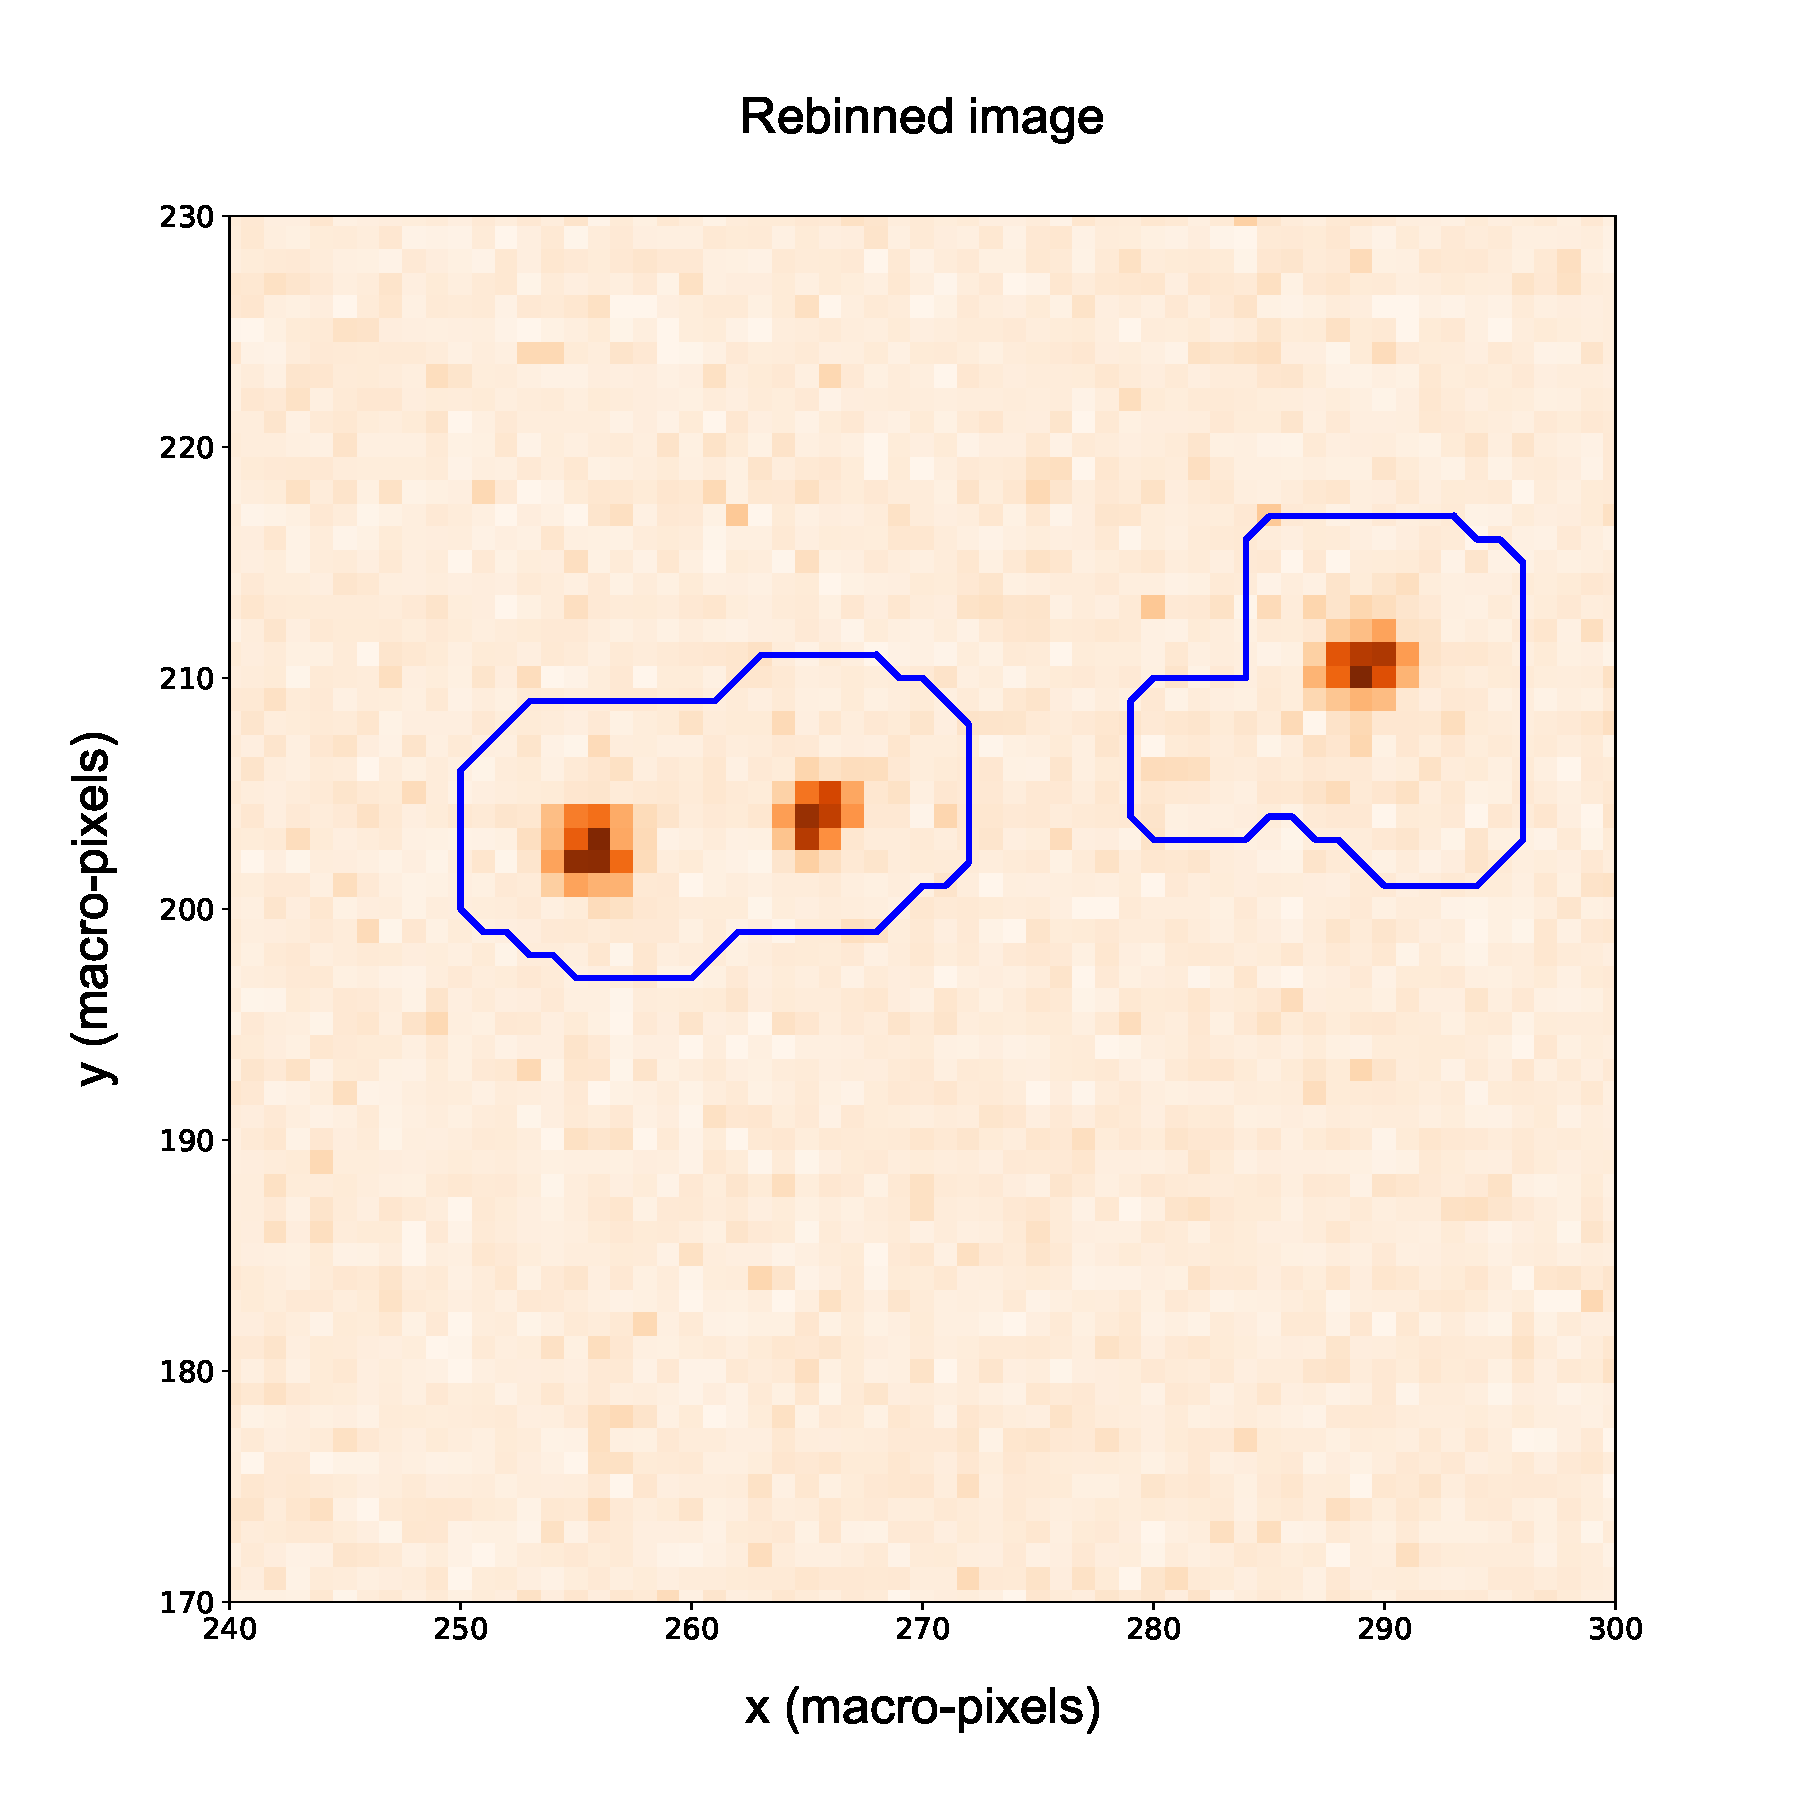
\includegraphics[width=0.49\linewidth]{figures/pic_run01843_ev93_2nd_3D_paper}
      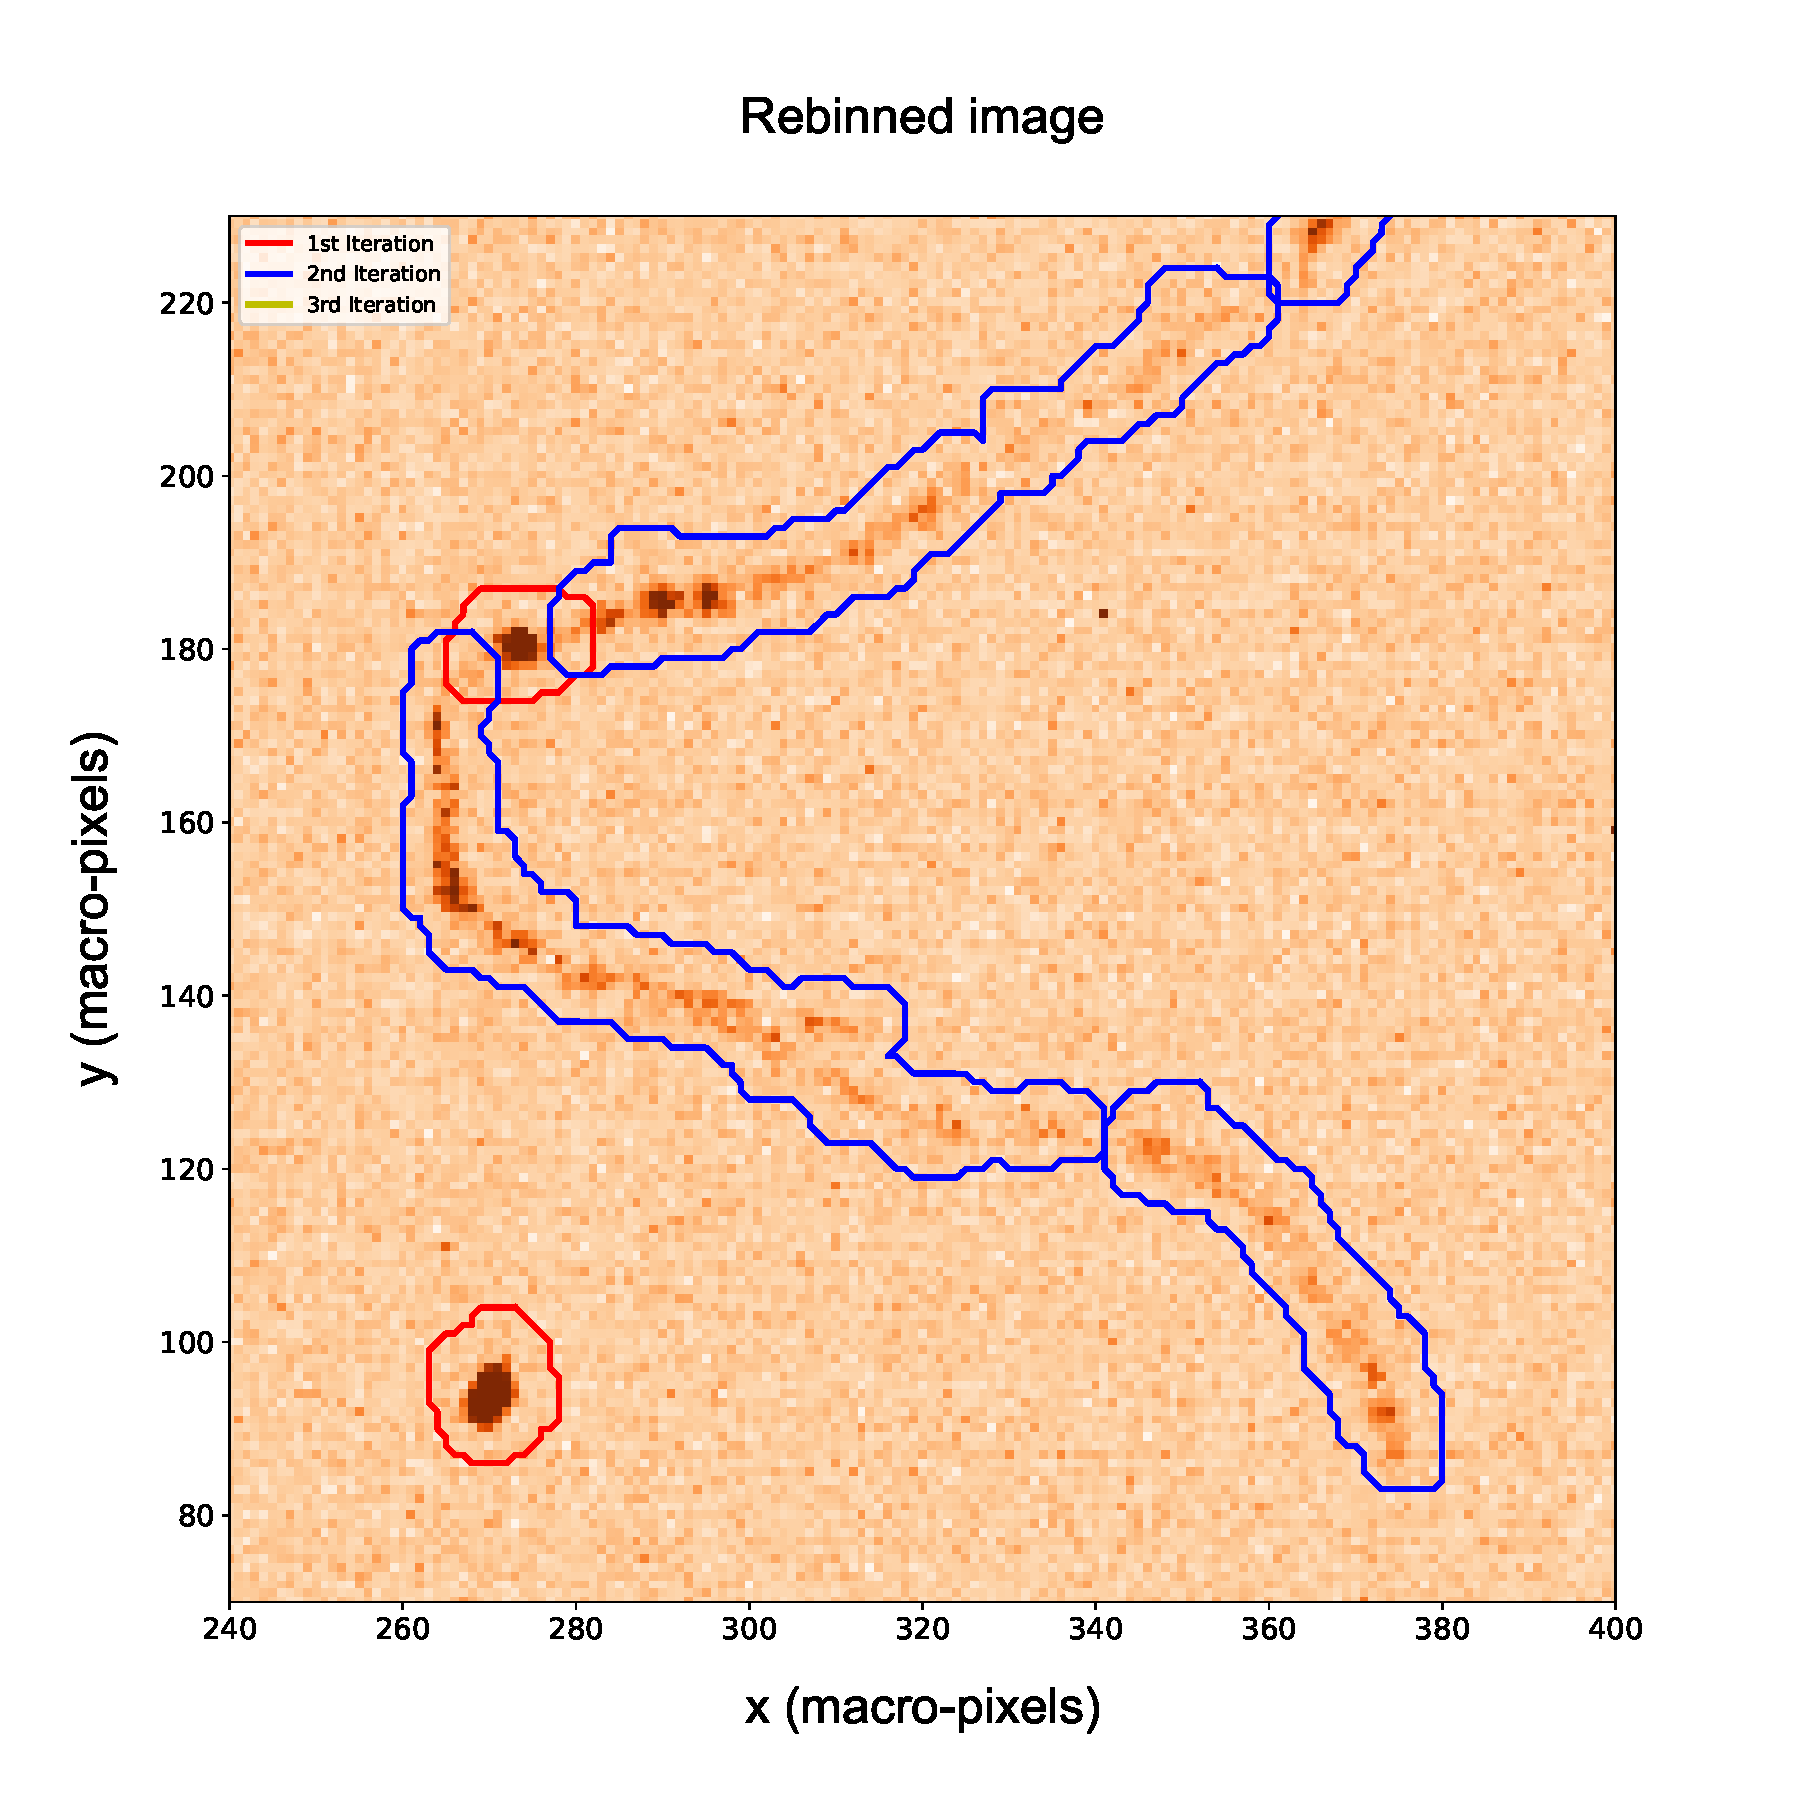
\includegraphics[width=0.49\linewidth]{figures/pic_run02317_ev8_all_3D_paper}
      \caption{Basic clusters reconstructed with the \idbscan
    algorithm in the low resolution (512$\times$512) image for two
    example events with very different patterns. Left: clusters on
    spots from \fe source, two of which are merged together. Right:
    Track from natural radioactivity and a nuclear recoil candidate in
    an event with \ambe source. The long track is split in several
    basic clusters of different \idbscan
    iteration. \label{fig:basic_clusters}}
  \end{center}
\end{figure}
